\chapter{Experimental methods} \label{chap:experimental}
% -------------------------
%% QUOTE
\vspace*{\fill}
\epigraph{As thou sowest, so shalt thou reap.}%
{\textit{De Oratore, II. 65. in Hoyt's New Cyclopedia Of Practical Quotations}\\ \textsc{Cisero}}
\clearpage{\thispagestyle{empty}\cleardoublepage}
%%
%% Body of the chapter
%%%%%%%%%%%%%%%%%%%%%%
This chapter provides an overview of experimental systems and procedures implemented in data acquisition throughout the project. Detailed description of used methods are given, where applicable, and their respective results are presented in Chapter \ref{chap:results}.

\section{PEC nanogels} \index{polyelectrolyte complex}
\subsection{Objective}
As explained earlier in Chapter \ref{chap:background}, a polyelectrolyte complex \index{polyelectrolyte complex} (PEC) is a nanoparticle that can be formed by mixing a polyanion and a polycation. Both constituents can be polymers with low molecular weights. Once the PEC is formed, an active ingredient (e.g. \ce{Cr^{3+}}) can be encapsulated into it, which will be later used to cross link polymers such as HPAM.

A research group at Texas A\&M\footnote{The research was originally conducted at University of Kansas. However, since Professor Jenn-Tai Liang, one of the contributors to this project and HyGreGel, later moved to Texas A\&M University, we will call it a Texas A\&M recipe here.} has developed a technology to delay gelation of HPAM based on PEC and \ce{Cr^{3+}}. Only a few works have been published on their results \citep[e.g.][]{Cordova2008,Johnson2010}. Figure \ref{cht:jennTai} shows an example of a system with delayed gelation based on Texas A\&M technology. As shown in the figure, the viscosity of the solution only increased marginally for the first 50 days after preparation. Then after 50 days, a sudden viscosity increase of several orders of magnitude was observed over a 10 day period.

As active amine POSS \index{amine POSS} nanoparticles are on type of polycations, it was proposed by Texas A\&M that amine POSS could possibly be used as polycation for PEC in the HyGreGel project. In this way there will be no need to add a third constituent as the nanoparticle also serves as the cross linker. This could possibly result in a more robust system for practical use as the system only includes two components. Initial measurements at Texas A\&M indicated that this could be a viable path to follow.

Therefore, several types of PEC nanogels were prepared and measured in order to test the idea.

\begin{figure}
    \centering
    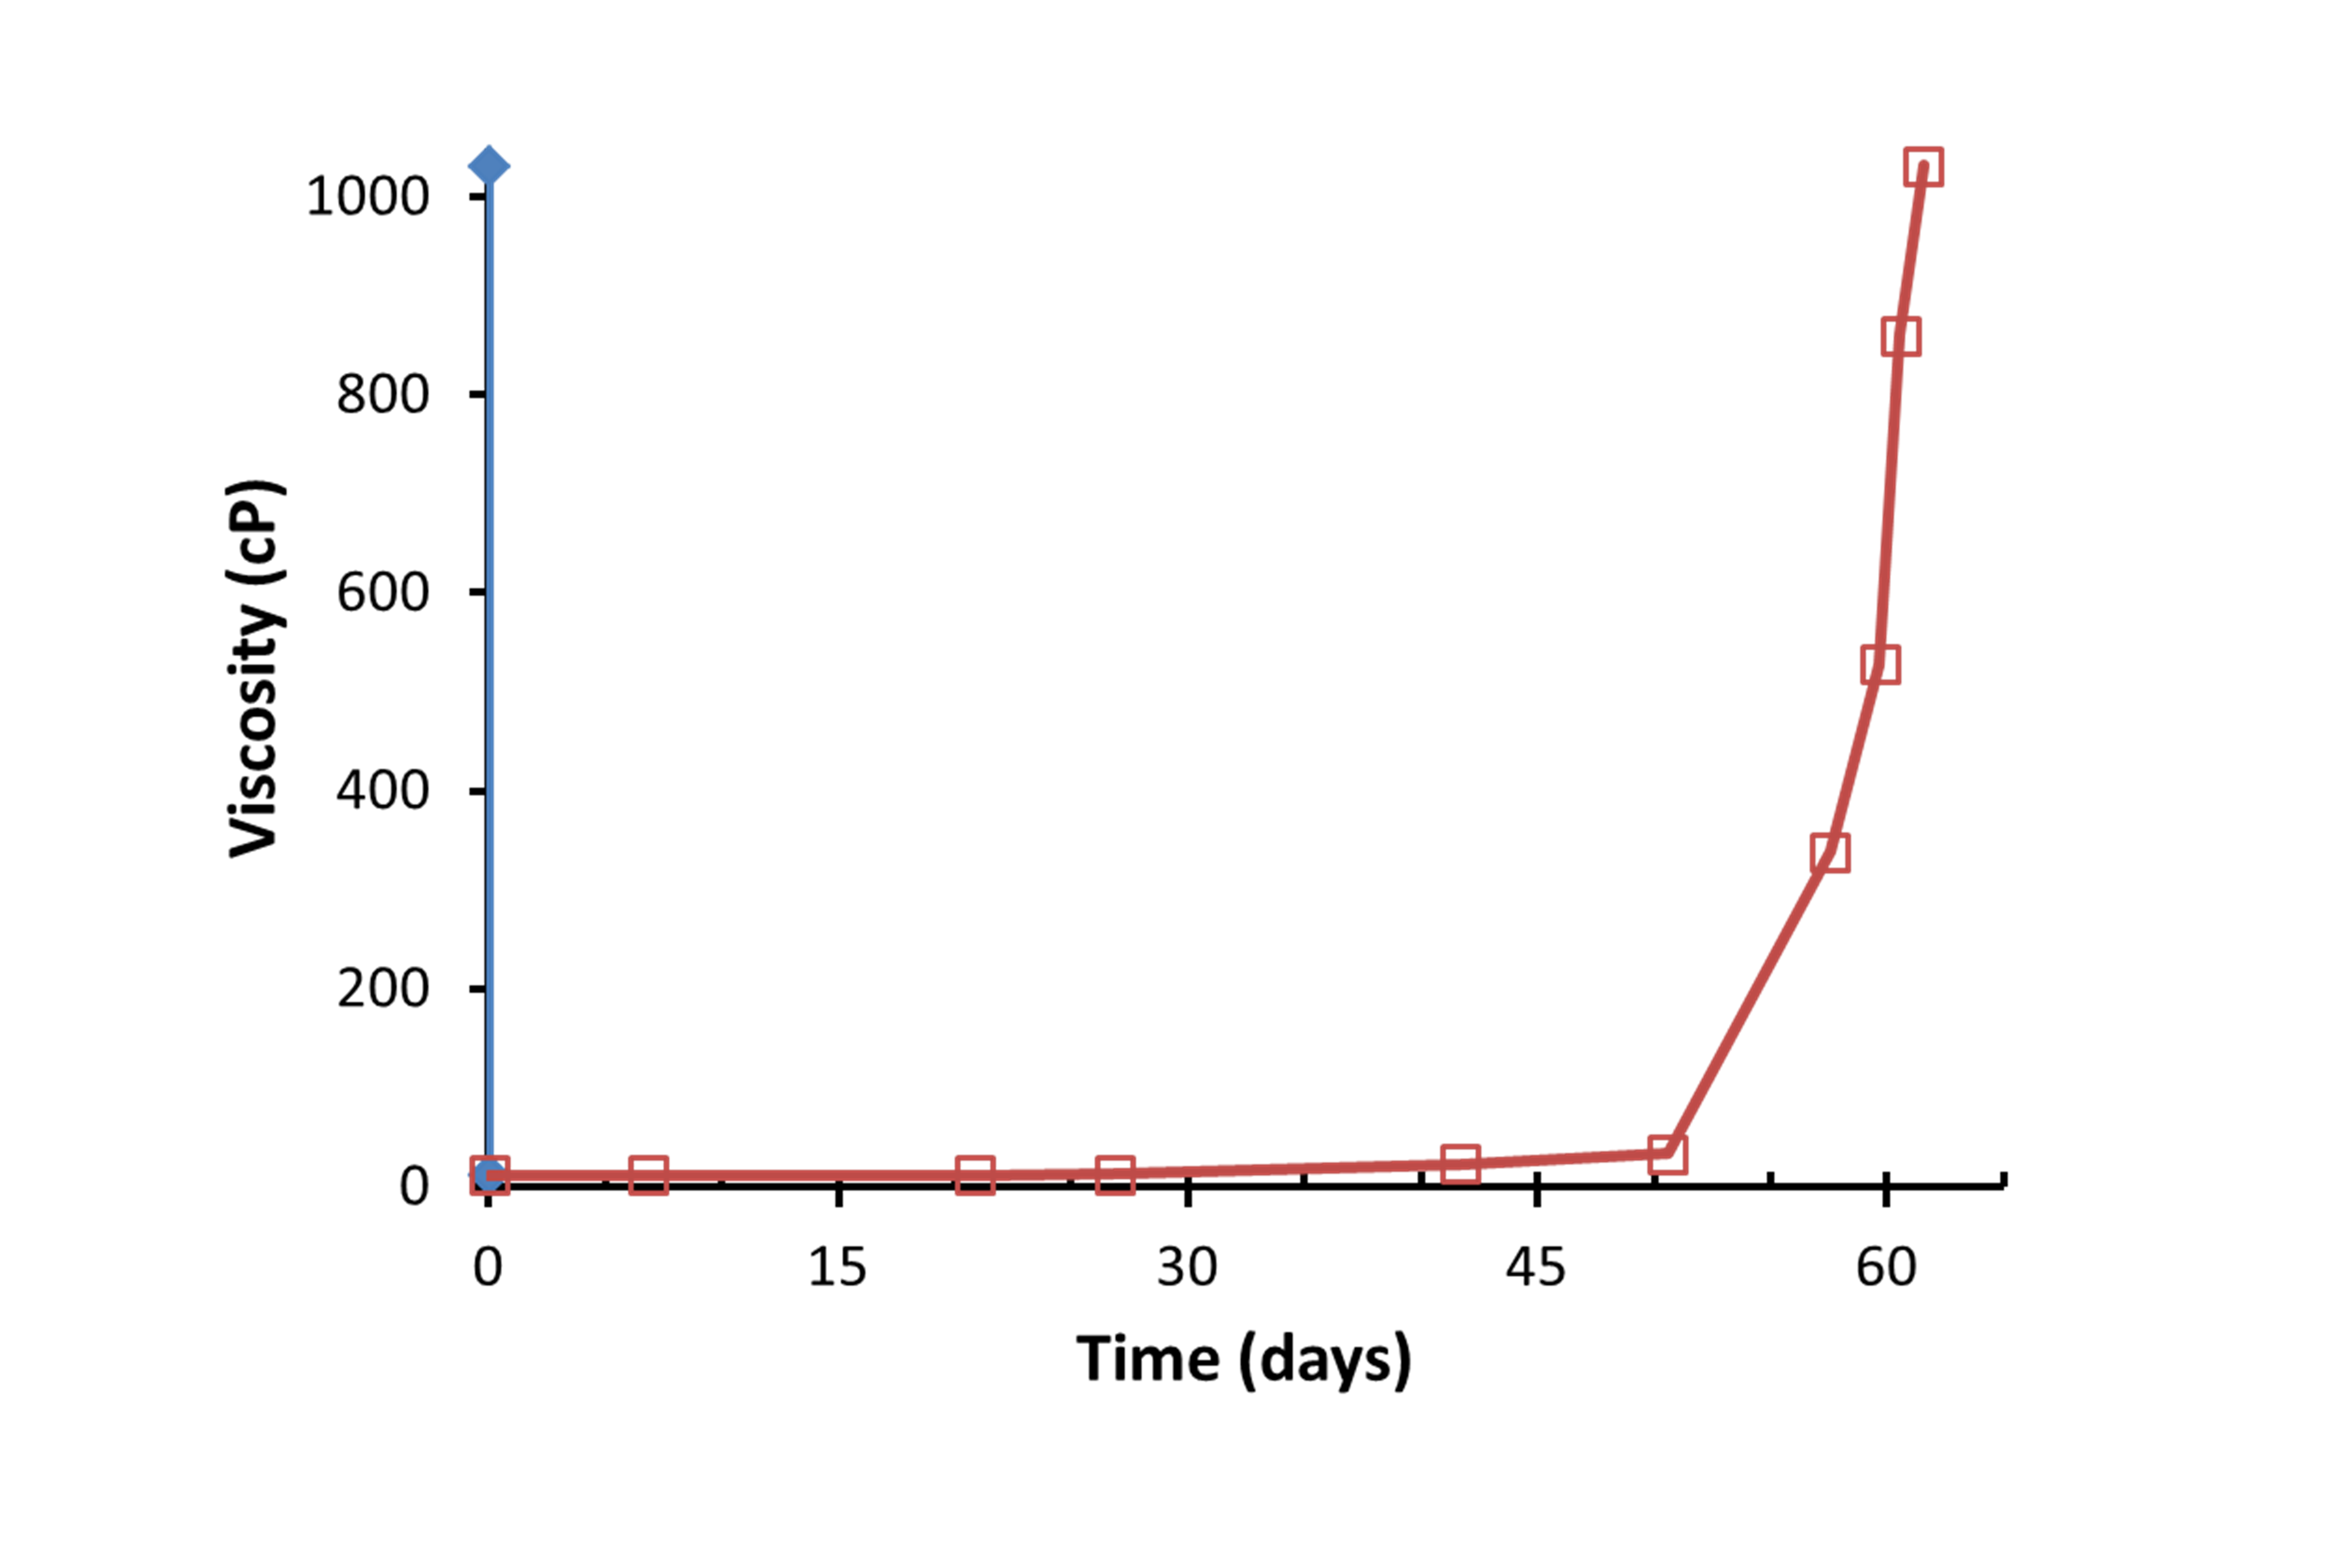
\includegraphics[width=.75\textwidth]{img/cht/jennTai.png}
    \caption{System with delayed gelation based on Texas A\&M technology \citep{Cordova2008}}
    \label{cht:jennTai}
\end{figure}

\newpage
The experiments on PEC nanogels consisted of three stages:
\begin{enumerate}
    \item Preparing the system in question (polymer and added components);
    \item Aging samples at elevated temperatures for various aging times;
    \item Measuring the viscosity of each sample at different shear rates.
\end{enumerate}

Appendix \ref{chap:gelSystem} includes a list of all the prepared gel systems as summarized in Table \ref{tab:gelSystemSummary}. Following the table are Figures \ref{fig:visc1-8} through \ref{fig:visc46}, which illustrate the viscosity behavior of the prepared systems versus time. 

\subsection{Preparation}

\subsubsection{Polymers and synthetic sea water}
\index{\ce{Cr^3+}} Three different polymers (all HPAM) were used in the experiments as summarized in Table \ref{tab:crGels}, where the product names, the producers and the approximate molecular weights are given. The concentrations used are also given. The polymers were always dissolved in synthetic sea water, SSW. Table \ref{tab:sswComp} shows the recipe for SSW used. The exact molecular weight of Flopaam 5115 VHM is not known but assumed to be in the order of 12 - 15 MDa.

\begin{table} 

\centering
\caption{Polymers used in the experiments}
\label{tab:crGels} % table 5.1
\begin{tabular}{c c c c } 
\toprule
\textbf{Name} & \textbf{Producer} & \textbf{MW} & \textbf{Concentration} \\ 
&& [MDa] & [wt\%]   \\
\midrule 
Alcoflood 254 S     & BASF    & 0.5 & 0.5, 1.0 and 2.0\\
Alcomer 24 UK       & BASF    & 6 & 0.25, 0.5, 1.0 and 2.0  \\ 
Flopaam 5115 VHM    & SNF Floerger    & 12 - 15 & 0.5, 1.0 and 2.0  \\ 

\bottomrule
\end{tabular}
\end{table}

\begin{table} 
\centering
\caption{Composition of synthetic seawater (SSW) \index{synthetic sea water}}
\label{tab:sswComp} 
\begin{tabular}{r c } 
\toprule
\textbf{Salt} & \textbf{Concentration} \\
& [g/l]\\
\midrule 
\ce{NaCl}       & 23.612\\
\ce{CaCl2.2H2O} & 1.911 \\ 
\ce{MgCl2.2H2O} & 9.149 \\ 
\ce{KCl}        & 0.746 \\
\ce{Na2SO4}     & 3.407 \\ 
\bottomrule
\end{tabular}
\end{table}

\subsubsection{Polyelectrolyte complexes according to the Texas A\&M recipe}
A few tests were conducted with PEC systems made after the recipe by \cite{Johnson2010}, in order to reproduce similar results. In this recipe, in addition to the polymer and cross binder \ce{Cr^3+} the main constituents are dextran sulphate (DS) \index{dextran sulfate} and polyethyleneimine (PEI)\index{polyethyleneimine}. The structure of the two polyelectrolytes are shown in Figure \ref{fig:pei}. Each molecule consists of n repeated units, but n is different for the two components. 1 wt.\% of both components in pure water were prepared for making PEC solutions by adding 15.39 g of DS solution to 34.28 g of PEI solution under vigorous stirring. The DS solution was added quickly as a ``shot" by use of a syringe.

\begin{figure}[h]
    \centering
    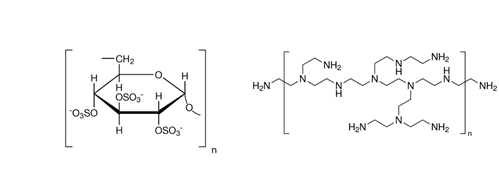
\includegraphics[width=\textwidth]{img/fig/pei.png}
    \caption{Structures of dextran sulphate (DS) (left) and polyethyleneimine (PEI) (right).}
    \label{fig:pei}
\end{figure}
 
After approximately one minute of stirring, 1.13 g of a 10 wt.\% \ce{CrCl3.6H2O} was added. The final solution was made by first mixing 5.38 g of a 4 wt.\% Alcomer 24 UK solution (in SSW\index{synthetic sea water}) with 25.35 g of SSW. Next, this polymer solution was mixed with 12.32 g of the PEC solution. The concentration of polymer and \ce{Cr^{3+}} in the final solution were 0.499 wt.\% and 129 ppm, respectively. The samples were aged at 50~\celsius. The sample series was named Series 10.

Two more series of polymer/PEC solutions were made using 0.498 wt.\% and 0.490 wt.\% of Alcomer 24 UK (Series 35) and Flopaam 5115 VHM (Series 36), respectively. The composition of the PEC was as described above. The concentrations of \ce{Cr^{3+}} in the two solutions were 119 ppm and 115 ppm. The solutions were aged at 80~\celsius. 

Yet another two systems were made in an equivalent manner using Alcomer 24 UK, but with reduced concentrations of \ce{Cr^{3+}} (60 ppm in Series 42 and 41 ppm in Series 47). Table \ref{tab:texasPecComp} shows a summary of prepared systems using the Texas A\&M recipe.

\begin{table} 
\centering
\caption{Composition of polymer/PEC sample series, concentrations in weight \%}
\label{tab:texasPecComp}
\begin{tabular}{c c c c c c } 
\toprule
\textbf{Sample} & \textbf{Polymer type} & \textbf{$C_{Polymer}$} & \textbf{$C_{Cr^{3+}}$} & \textbf{Aging temperature}  \\ 
& &[wt\%]& [ppm] & [\celsius] \\
\midrule 
Series 10   & Alcomer 24 UK         & 0.499 & 129 & 50\\
Series 35   & Alcomer 24 UK         & 0.498 & 119 & 80\\ 
Series 36   & Flopaam  5115  VHM    & 0.490 & 115 & 80\\ 
Series 42   & Alcomer 24 UK         & 0.498 & 60  & 80\\
Series 47   & Alcomer 24 UK         & 0.499 & 41  & 80\\
\bottomrule
\end{tabular}
\end{table}

\subsubsection{Polyelectrolyte complexes based on amine POSS}\index{polyhedral oligomeric silsequioxanes}

\index{amine POSS} In PECs based on amine POSS the polycation PEI was replaced by the nanoparticle which also contains amine groups. As suggested by researchers at Texas A\&M the DS was replaced by the polyanion polyvinyl sulfonate (PVS)\index{polyvinyl sulfonate}. Series 17 through 20 were made using this method (Table \ref{tab:polyPecComp}). The structure of PVS is also shown in Figure \ref{fig:pvs}.

\begin{figure}[h]
    \centering
    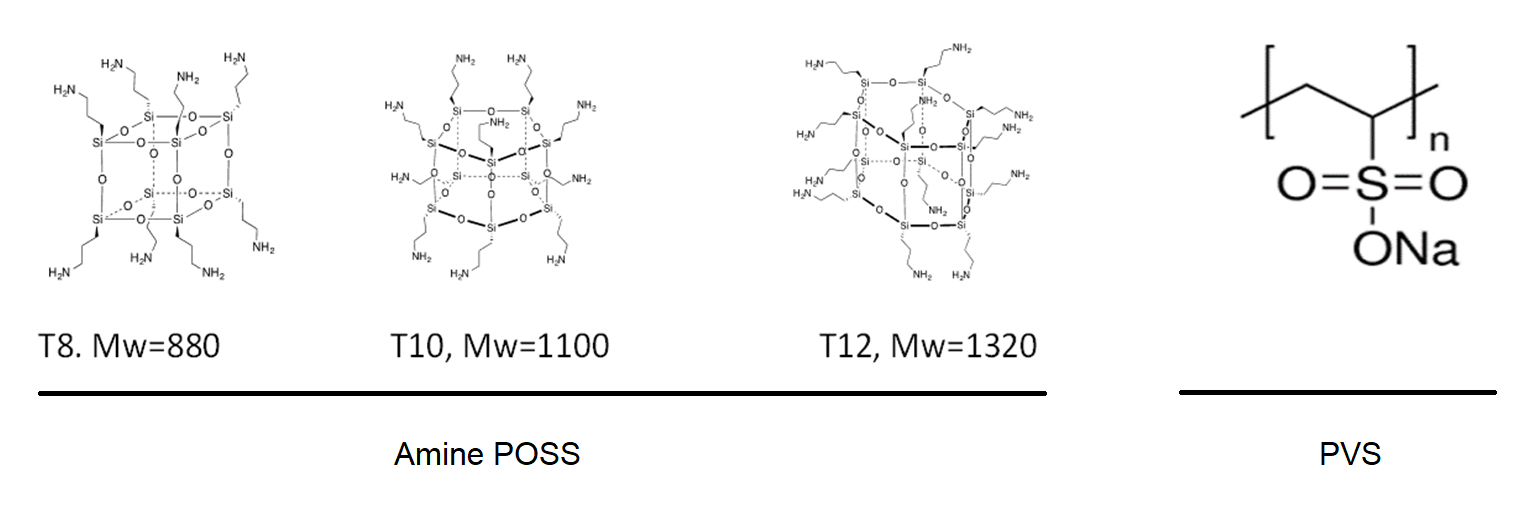
\includegraphics[width=\textwidth]{img/fig/pvs.png}
    \caption{Structures of amine POSS (left) and PVS (right).}
    \label{fig:pvs}
\end{figure}

The cores of the amine POSS are silicon oxide. The structure of the cores varies with the configurations shown in the figure, giving different molecular weights of the POSS particles. The amide POSS particles used in the samples were labelled FN 161128 and was 64.63 \% active matter in solvent.

Alcomer 24 UK was used as polymer. The composition of the samples are summarized in Table \ref{tab:polyPecComp}. The solvent for the solutions was SSW.

\begin{table} 

\centering
\caption{Composition of polymer/PEC sample series, concentrations in weight \%}
\label{tab:polyPecComp}
\begin{tabular}{c c c c c c } 
\toprule
\textbf{Sample} & \textbf{$C_{Polymer}$} & \textbf{$C_{FN}$} & \textbf{$C_{PVS}$} & \textbf{$C_{pol}/C_{FN}$} & \textbf{$C_{FN}/C_{PVS}$} \\ 
&[wt\%]& [wt\%] & [wt\%] && \\
\midrule 
Series 17   & 1.002   & 0.380 & 0.053 & 2.64 & 7.16\\
Series 18   & 1.004   & 0.381 & 0.136 & 2.64 & 2.80\\ 
Series 19   & 0.931   & 0.382 & 0.273 & 2.64 & 1.29\\ 
Series 20   & 1.000   & 0.436 & - & 2.30     & - \\
\bottomrule
\end{tabular}
\end{table}

\subsubsection{Gels based on lactamide POSS}
% The development of gel systems based only on functional nanoparticles giving delayed gelation was described in Chapter \ref{chap:materials}. In this section measurement of samples taken during injection of nanoparticle/polymer system used in the in-situ gelling experiments described in Section 5.3 are shown. 

\index{lactamide POSS} The solutions used in the core flooding experiments were prepared by mixing 500 g of 2 wt. \% Alcoflood 24 UK with 17.35 g of the lactamide POSS FN-LA-65-170210-1. The nanoparticles were supplied as a 90.59 \% active solid.

During the core flooding experiments the nanoparticle/polymer solution was injected into the SSW saturated cores. The viscosity of the effluent was monitored. As soon as the effluent viscosity had stabilized, a series of samples were taken. Furthermore, towards the end of the injection more samples were taken. After collection and argon-purging, the samples were aged at 80~\celsius. 

\subsection{Aging}
Each prepared system was distributed into six vials (a through f) that were sealed with rubber stoppers and crimp seals, as shown in Figure \ref{fig:vials}. Then the vials were placed on a KS 500 shaker (Janke \& Kunkel, IKA WERK, Figure \ref{fig:shaker}) with 300 shakes/min. While being shaken, the vials were purged with argon for 60 minutes. Argon was delivered through a syringe needle penetrating the rubber gasket. It then exited the vial through another needle (see Figure \ref{fig:argonPurge}).
\begin{figure}[p]
    \centering
    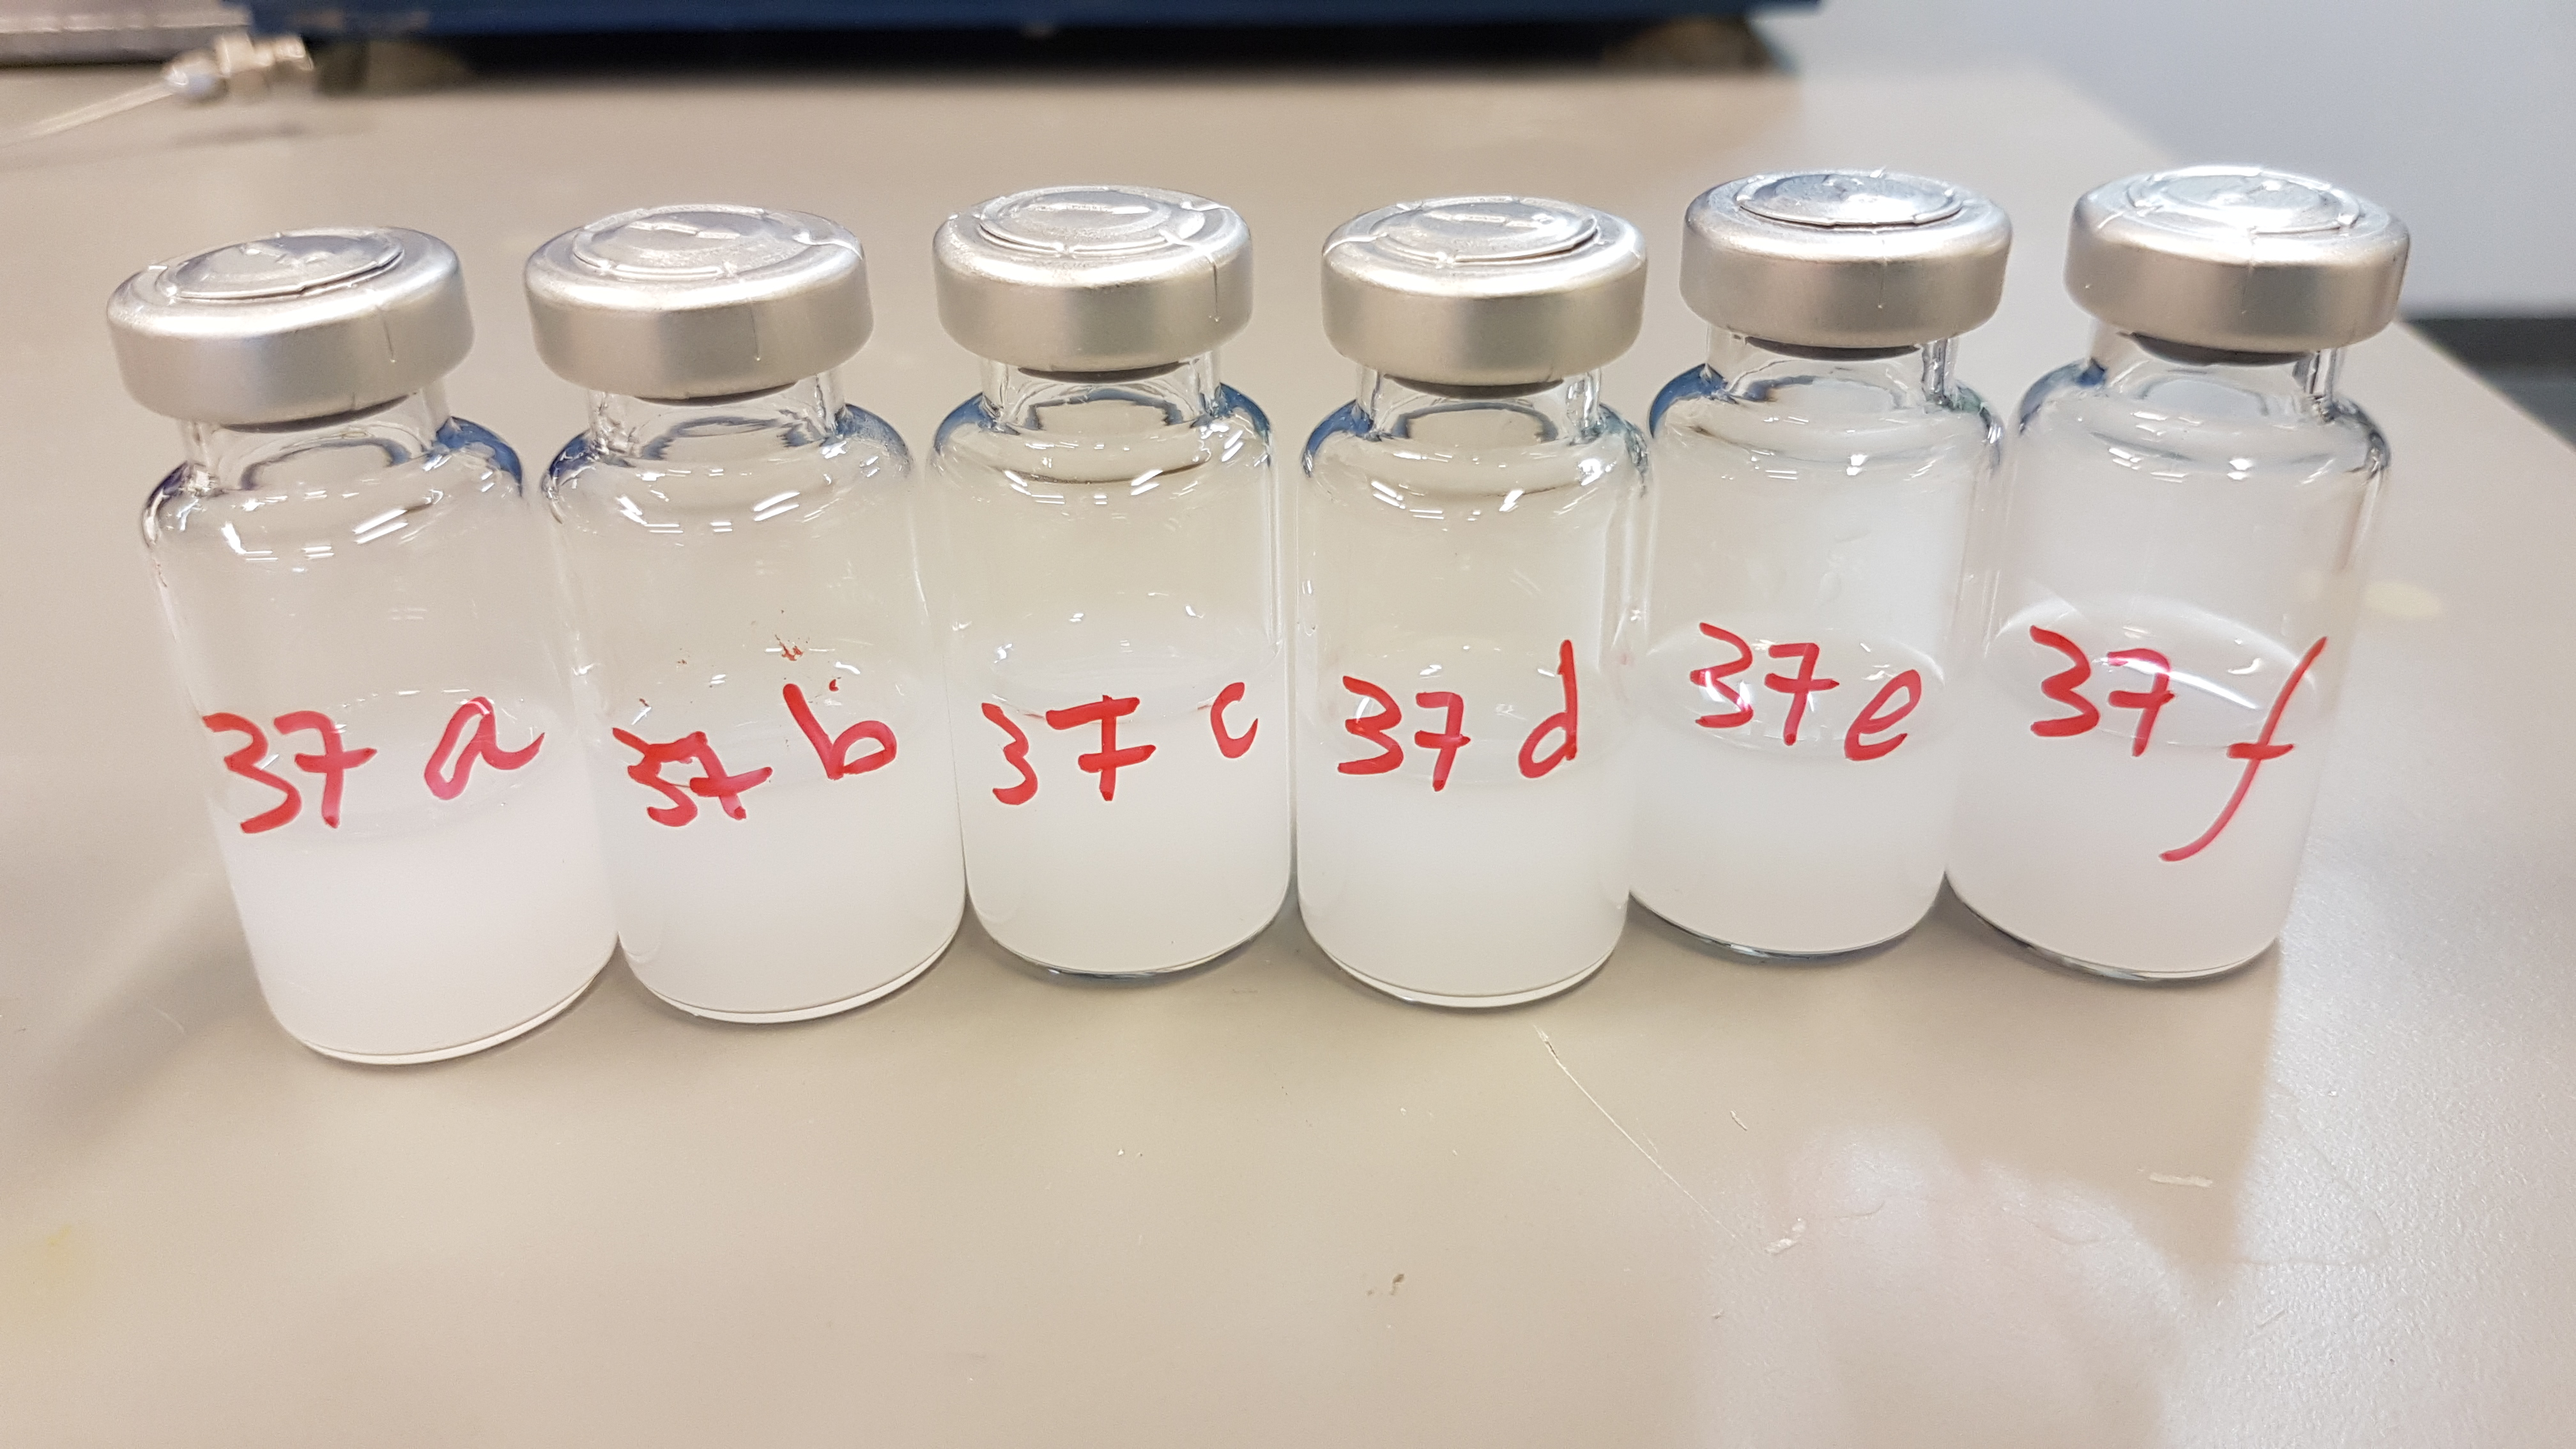
\includegraphics[width=.7\textwidth]{img/fig/vials.jpg}
    \caption{System \#37 distributed into vials ``a" through ``f" with rubber stoppers and crimp seals}
    \label{fig:vials}
\end{figure}
\begin{figure}[p]
    \centering
    \begin{subfigure}{0.45\textwidth}
        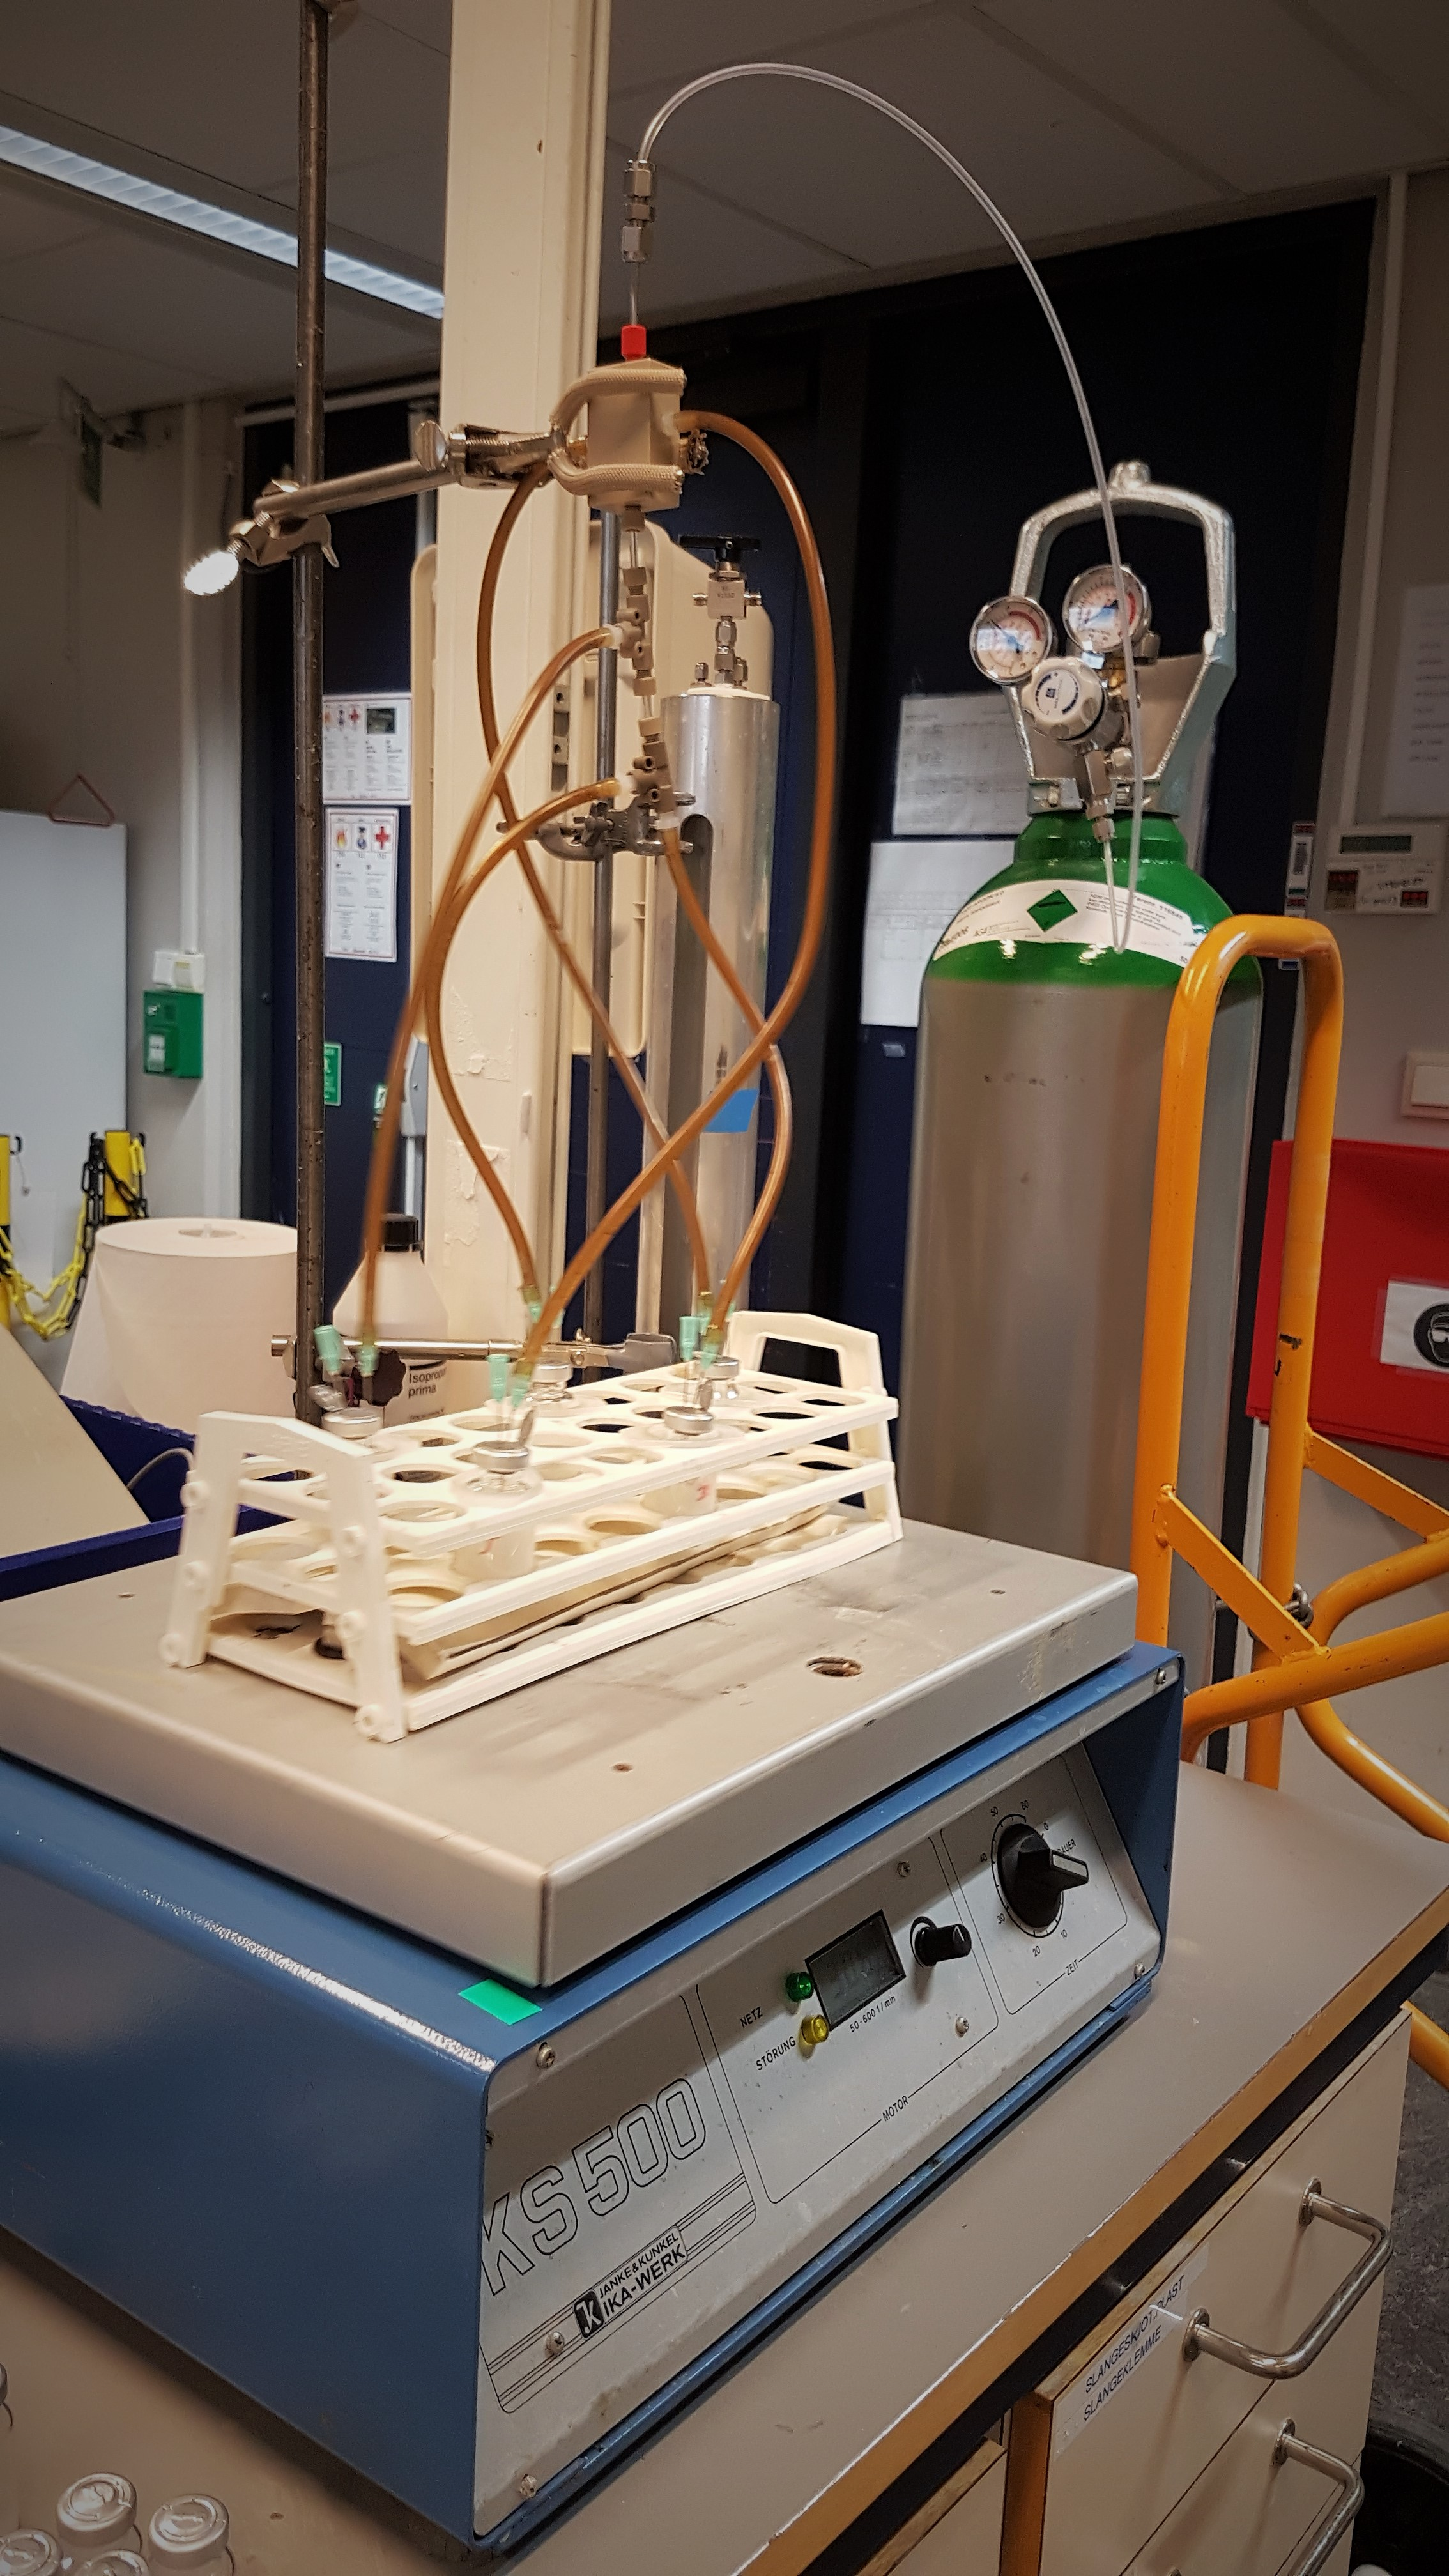
\includegraphics[width=\linewidth]{img/fig/shaker.jpg}
        \caption{} \label{fig:shaker}
    \end{subfigure}
    \hspace*{.05\textwidth} % separation
    \begin{subfigure}{0.45\textwidth}
        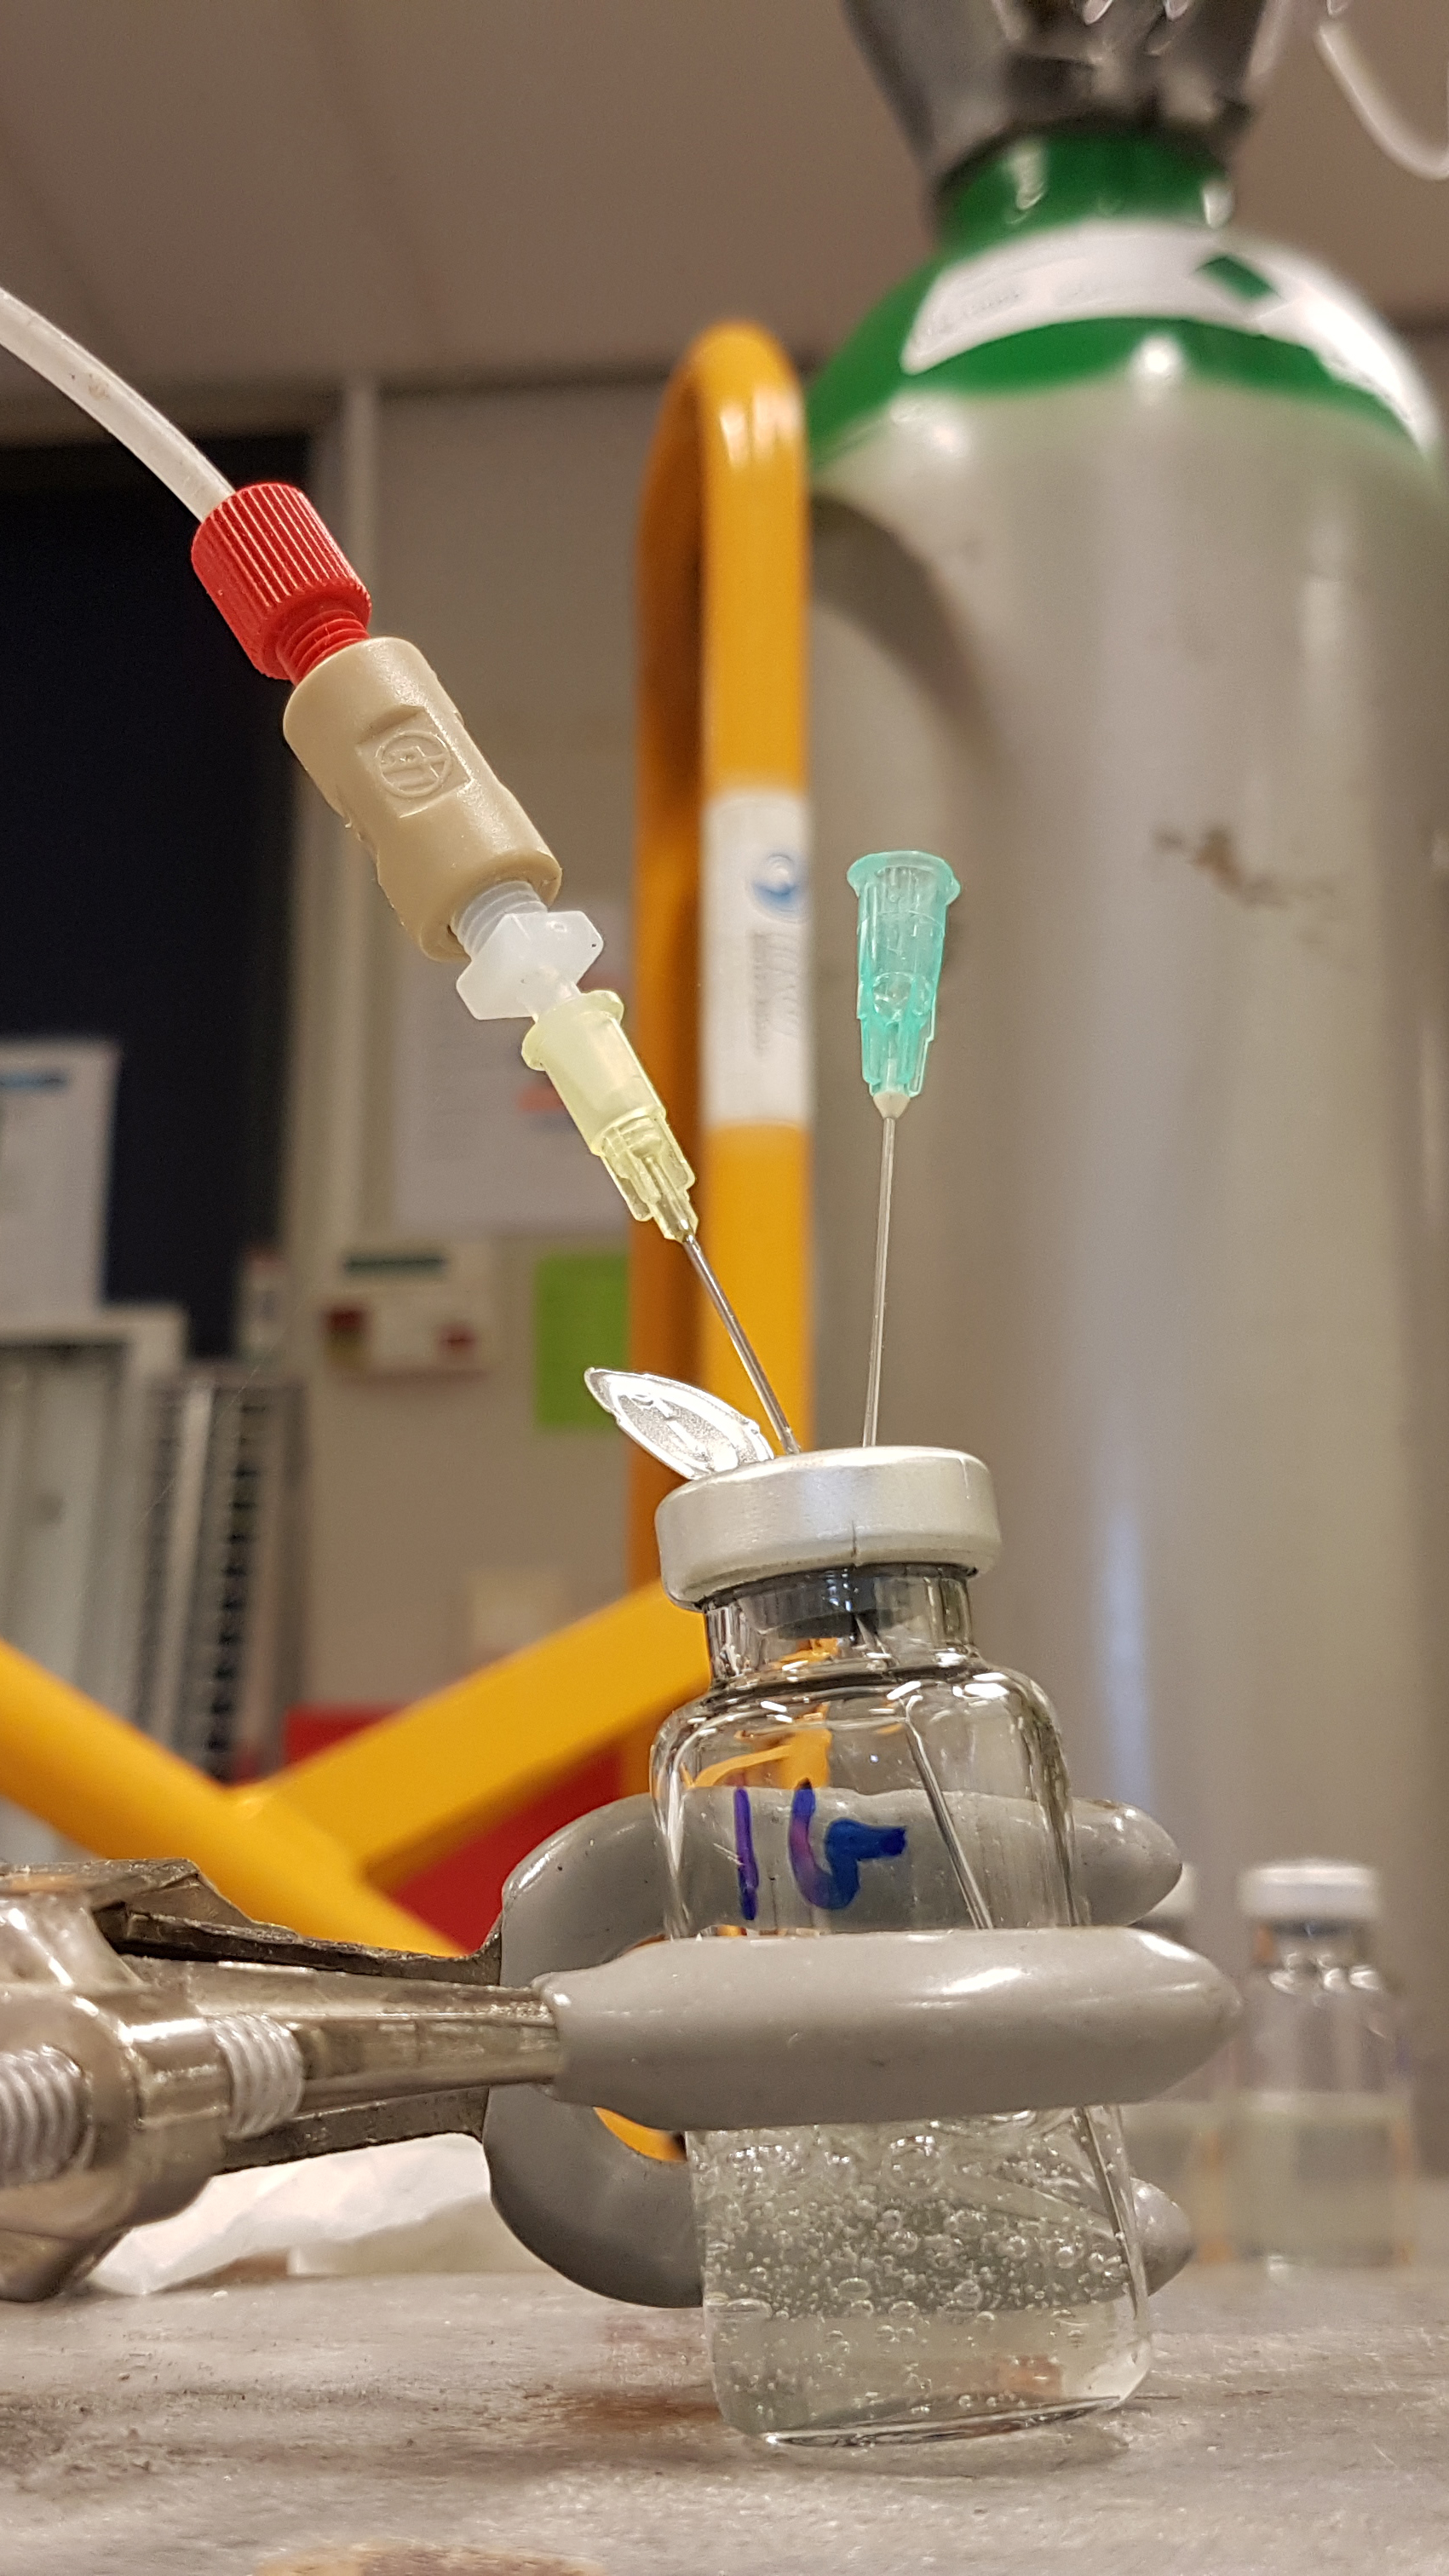
\includegraphics[width=\linewidth]{img/fig/argonPurge.jpg}
        \caption{} \label{fig:argonPurge}
    \end{subfigure}
    \caption{Purging samples with argon over a KS 500 shaker. (a) Shaker and argon cylinder (b) Argon purging syringe system with input and output needles}
    \label{fig:shaking}
\end{figure}

After the purging, samples were placed in an oven and were heated to 50~\celsius~(the first 16 series) and later at 80~\celsius. The ``a" sample from each series was not heated, and its viscosity was measured a short time after preparation. Samples ``b" through ``f" were kept in the oven, each for an exponentially increased aging time. 

\subsection{Viscosity measurement}
The \index{viscosity} viscosities of samples were measured using an Anton Paar MCR 302 rheometer (Figure \ref{fig:antonPaar}) under ambient conditions. After a sample was taken out of the oven, it was quickly transferred to the rheometer station, after which its viscosity was measured using a plate and cone geometry.

\begin{figure}[h]
    \centering
    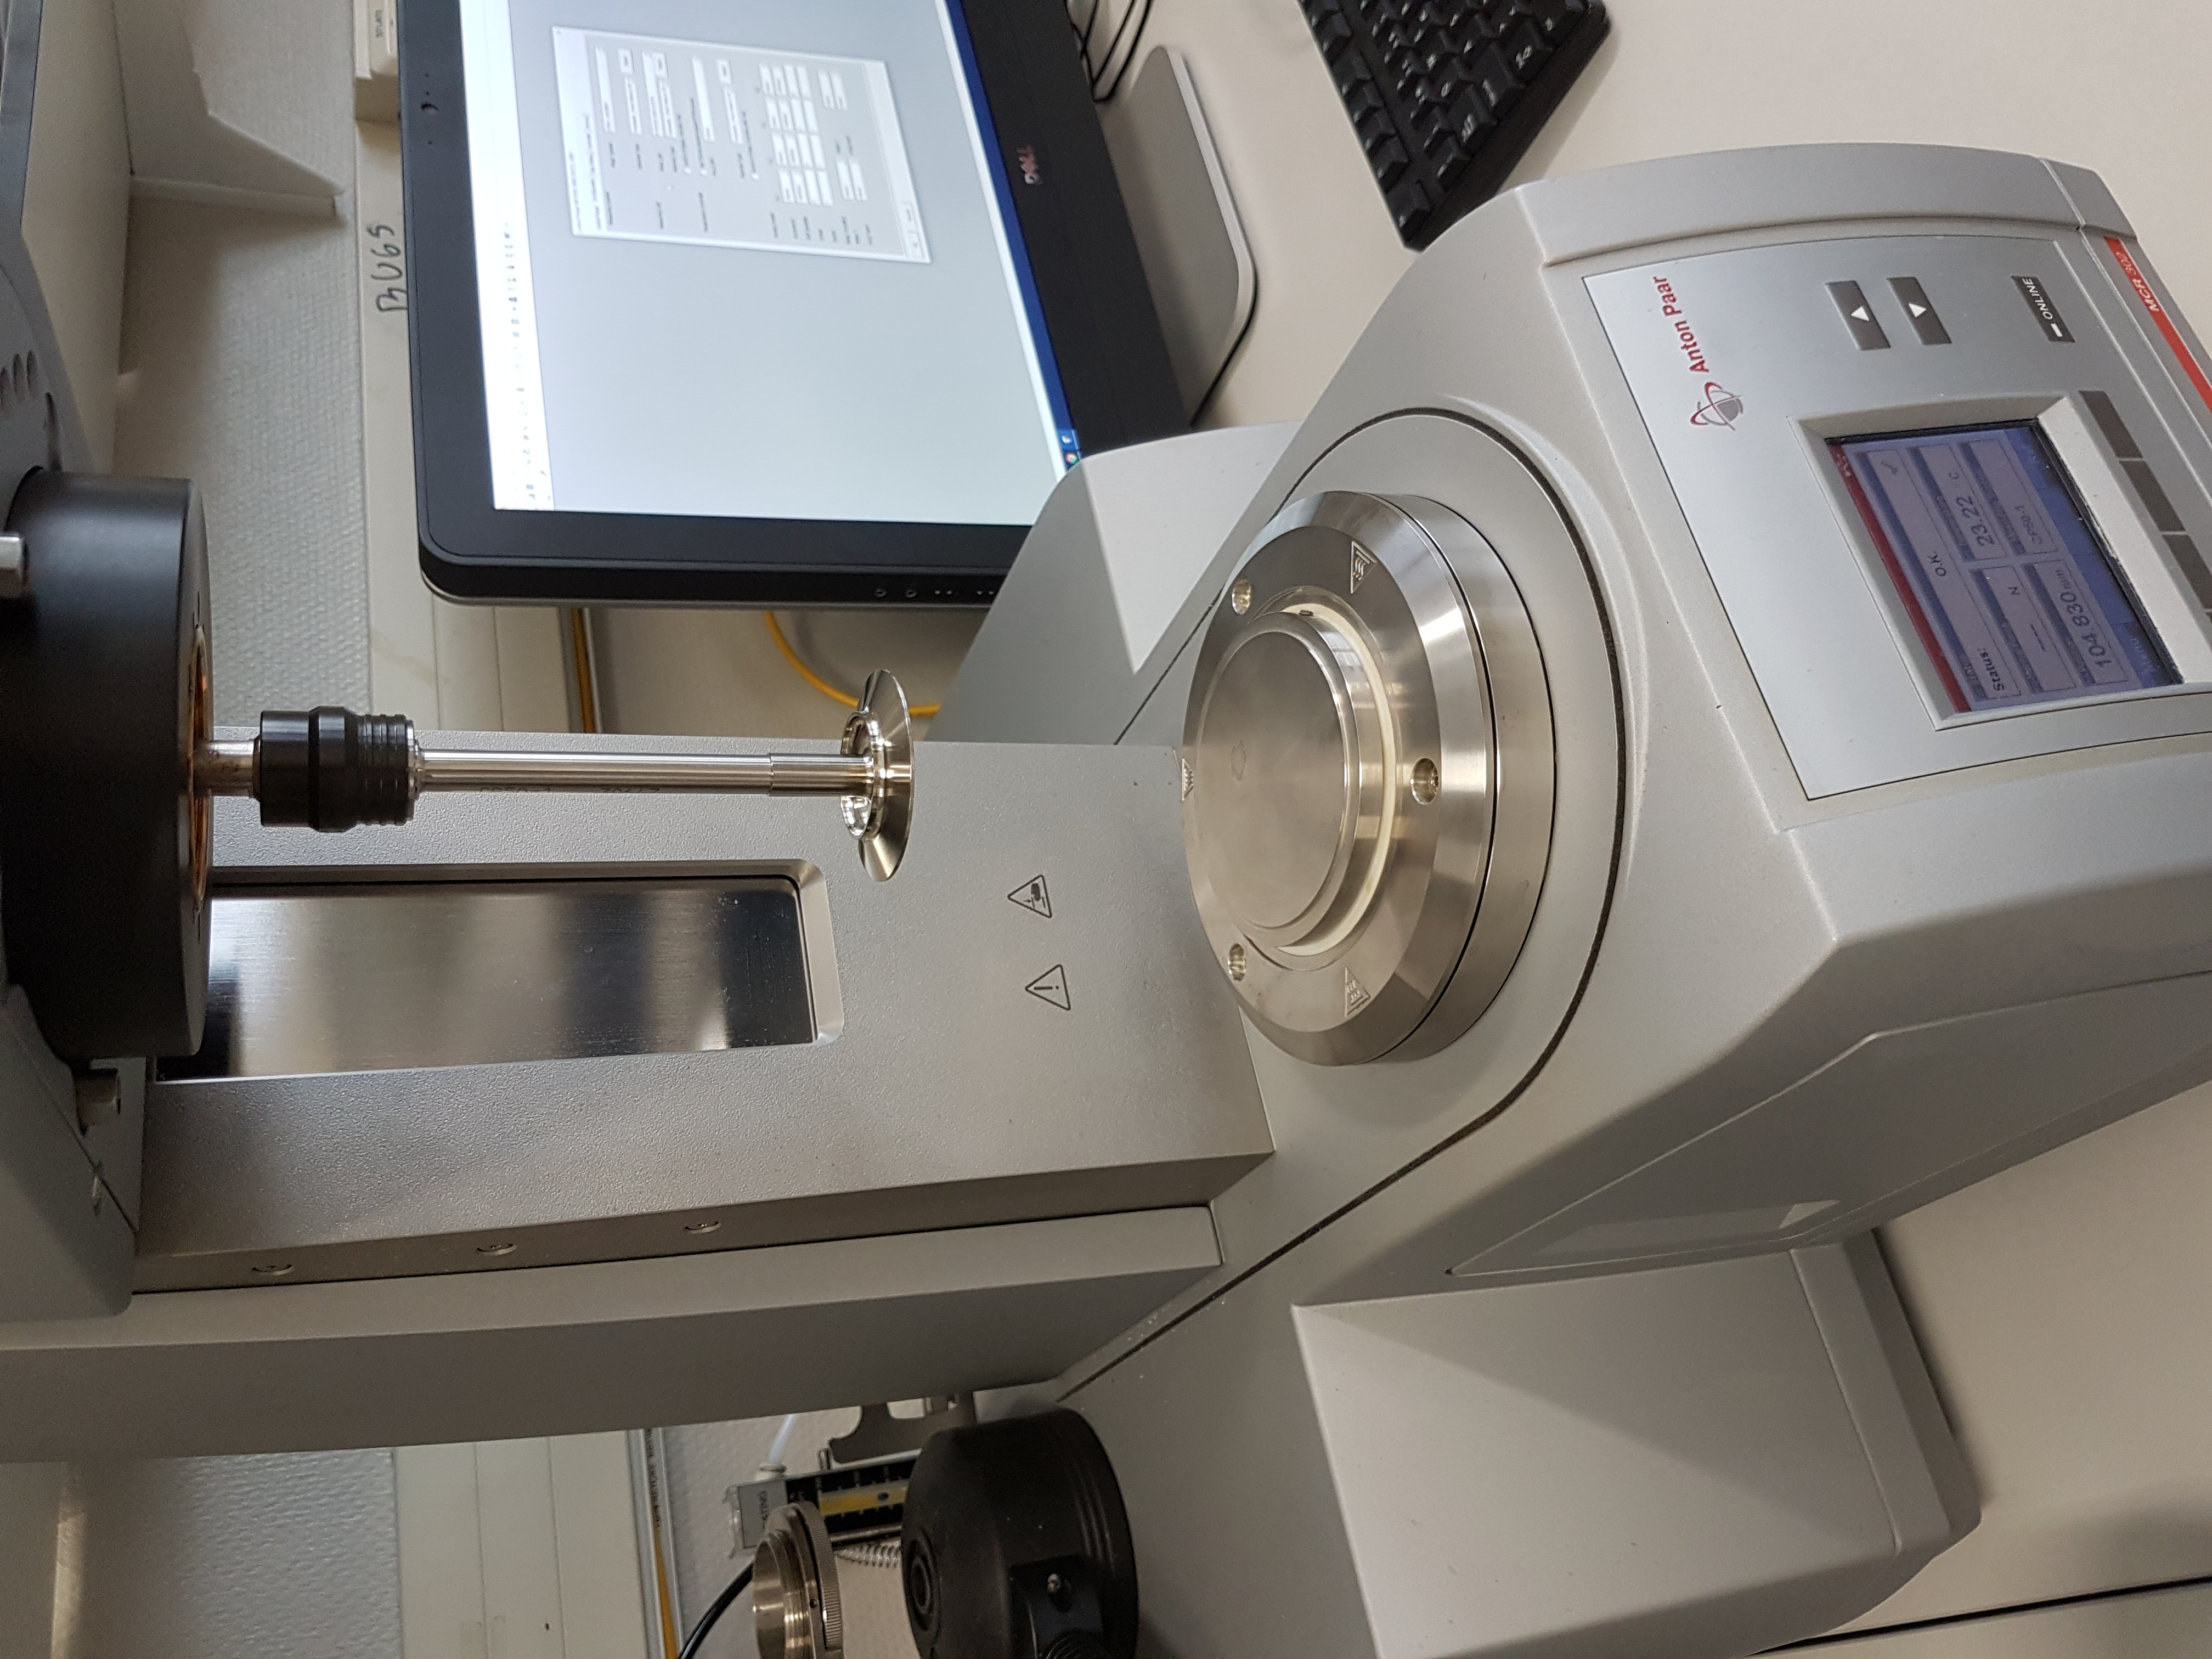
\includegraphics[width=.5\textwidth, angle=270]{img/fig/antonpaar.jpg}
    \caption{Anton Paar MCR 302 rheometer}
    \label{fig:antonPaar}
\end{figure}

The measurement procedure using the rheometer is as follows. First, a sample of suitable size was put on the plate. After that, the cone was lowered down onto the sample, until the sample spread into a thin film which completely filled the space between the cone and the plate. The measurement was then started according a preset schedule for shear rates. 

After initiating measurements, the instrument imposed a torque on the plate by rotating the cone at an initial slow speed, which was necessary to apply the first shear rate. The rotation lasted for the measurement time which was set to 2 seconds. After the measurement time had elapsed, the torque was increased to reach the next shear rate. The shear rates ranged from $10^{-3}$ to $10^{3} (\text{s}^{-1})$, and 20 measurements with exponential increase in shear rates were made within this range. From the resulting torques and shear rates a relationship between viscosity and shear rate (shear curve) was then calculated by the software.

Admittedly, measuring shear curves is not the ultimate way of characterizing gel systems after gelation has started. Weak gels may be broken down during the shearing. For stronger gels, the velocity gradient between the measuring geometry will not be as homogeneous as in a weaker, more fluid gel, since it will only be over a small gap between the measurement bodies (cone and/or plate) and the gel. For such systems, other types of measurements can be used to get more accurate results, \textit{e.g.}, oscillatory measurements. Thus, the measurements presented in this chapter are at best semi-quantitative after gelation had started. However, valuable results were collected from said measurements.

Some operational issues arose in the process. For some systems, after gels were formed, it was difficult or impossible to remove the gel from the vial. After extracting such samples from vials, it was possible to obtain a shear curve for some systems. Other systems would not stay in place and slipped away when the cone was lowered onto the sample on the plate.

\section{Transport of polymer and nanoparticles through porous media}
\subsection{Objective}
The \index{transport in porous media} objective of these series of experiments was to investigate the transport properties of the chemical systems in the project through porous media.To this end, several core flooding experiments were conducted.

\subsection{Experimental setup}
A schematic of the experimental setup \index{experimental setup} is shown in Figure \ref{fig:experimentalSetup}. To the right of the setup there were reservoirs containing either SSW, nanoparticle solution, polymer solution or mixtures of the latter two. The solutions were then pumped by a dual piston Pharmacia P-500 pump, and injected into the bottom of the vertical oriented core. The core itself was wrapped in nickel foil and inserted into a Viton rubber sleeve, around which a net overburden pressure of 50 bar was exerted. This ensured that no side flow occurred around the core and the metal foil prevented the sleeve pressure gas to diffuse through rubber sleeve.

\begin{figure}[hp]
    \adjustbox{minipage=\textheight,angle=90}{
        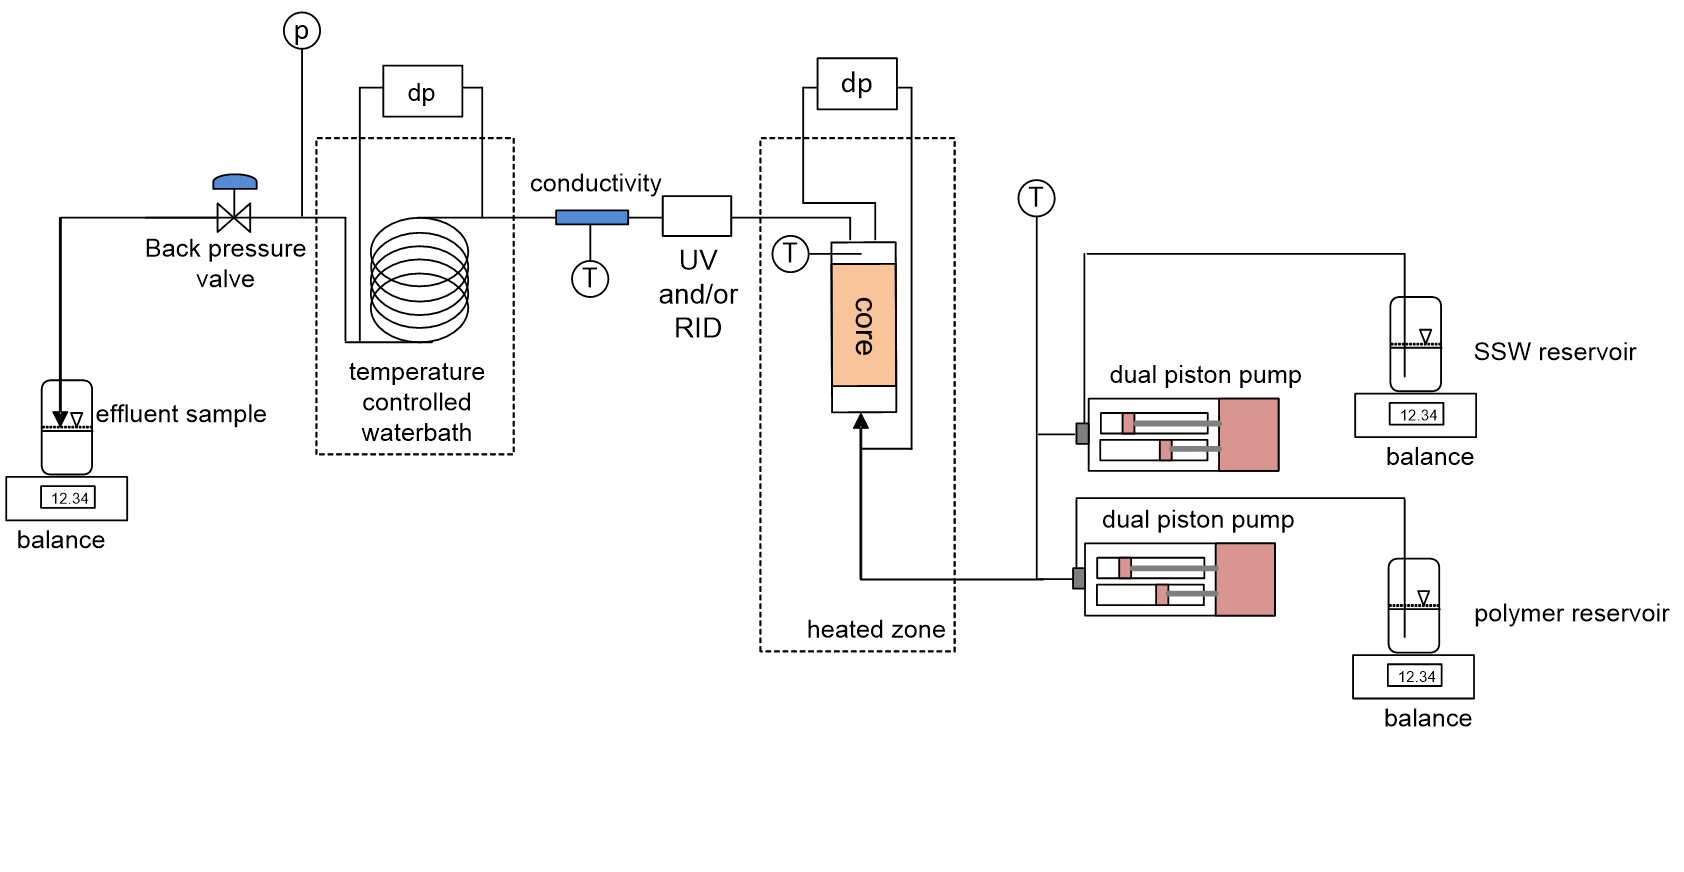
\includegraphics[width=\textwidth]{img/fig/experimentalSetup.png}
        \caption{Schematic of the setup of the core flooding experiments.}
        \label{fig:experimentalSetup}
    }
\end{figure}

Several online measurement systems were placed downstream of the core. Conductivity of the effluent was measured by a Radiometer CDM 83 Conductivity Meter, determining the resistance of the fluid between two small rodded platinum electrodes integrated in a flow channel in a small housing made of polyoxymethylene. Since conductivity is substantially affected by temperature, these readings were temperature corrected. Viscosity of the effluent was measured by a spiral viscometer of 1/16" outer diameter. In order to avoid temperature effects, the viscometer was submerged in a water bath with a constant temperature. A refractive index detector (Shodex RI SE-51) and UV detector (KNAUER Azura MWD 2.1L) were employed interchangeably, in order to determine nanoparticle concentration. Several pressure transducers were implemented along the system. A back pressure of 3 – 6 bar was applied. To the left side of the experimental setup, the effluents were collected and weighed. The core temperature was at ambient for the experiments described in this section.

\subsection{Core flooding experiments with polymer and/or inactive FN particles}

First, \index{core flooding} a new core of diameter 3.8 cm and length 20 cm, was mounted in the core holder. After leakage testing of the system, the core was flooded with isopropanol until full saturation. Next several PVs of synthetic seawater (SSW) were flooded through the core in order to displace the isopropanol and ensure stable flow conditions. After that, porosity and permeability measurements were conducted. Porosity was measured by NaNO3 flooding of the SSW saturated core. The concentration of \ce{Cl-} in the collected fluid was determined by potentiometric titration. The pore volume (PV) was calculated from the total amount of chloride, adequately corrected for dead volumes.

Each experiment started with injection of a slug with only nanoparticles, only polymer or a mixture of nanoparticles and polymer (Stage 1). After some time, the measurements stabilised. In Stage 2, the injected fluid was switched to pure brine (with lower salt concentration in the experiments only involving polymer) and the injection continued until the measurements became stable. In Stage 3, a second slug with additives was injected, followed by a second slug with only brine (Stage 4). In other words, stages 3 and 4 were a repetition of stages 1 and 2. All stages ran until measurements became steady state. The experiment ended with a final water permeability measurement. During the experiment, process parameters and detector/sensor readings were continuously logged.

Quantification of produced polymer and nanoparticles was carried out using the viscosity measurements and/or measured changes in refractive index and UV absorption. Figure \ref{cht:uv} shows calibration models for UV absorption \index{UV absorption} and pressure drop in the viscometer tube. As seen in the figure, the pressure drop over viscometer tube is practically only affected by polymer concentration, giving a second order model in polymer concentration. Viscosity measurements alone were therefore used to find the concentration of produced polymer. On the other hand, UV absorption data resulted in a model with first and second order terms with respect to both nanoparticles and polymer, as well as a cross term (i.e., the product of concentrations). Similar responses were also found for changes in \index{refractive index} refractive index. UV absorption measurements and changes in refractive index were used to generate nanoparticle responses. For the experiments that involved nanoparticles, the conductivity responses were determined in separate runs from the main core floods. This was because changes in salt concentration affected both UV absorption at low wavelengths and especially the refractive index of the fluid. The conductivity responses were measured with the same injection rates with slugs of SSW and 80\% SSW into the cores.

\begin{figure}[h]
    \centering
    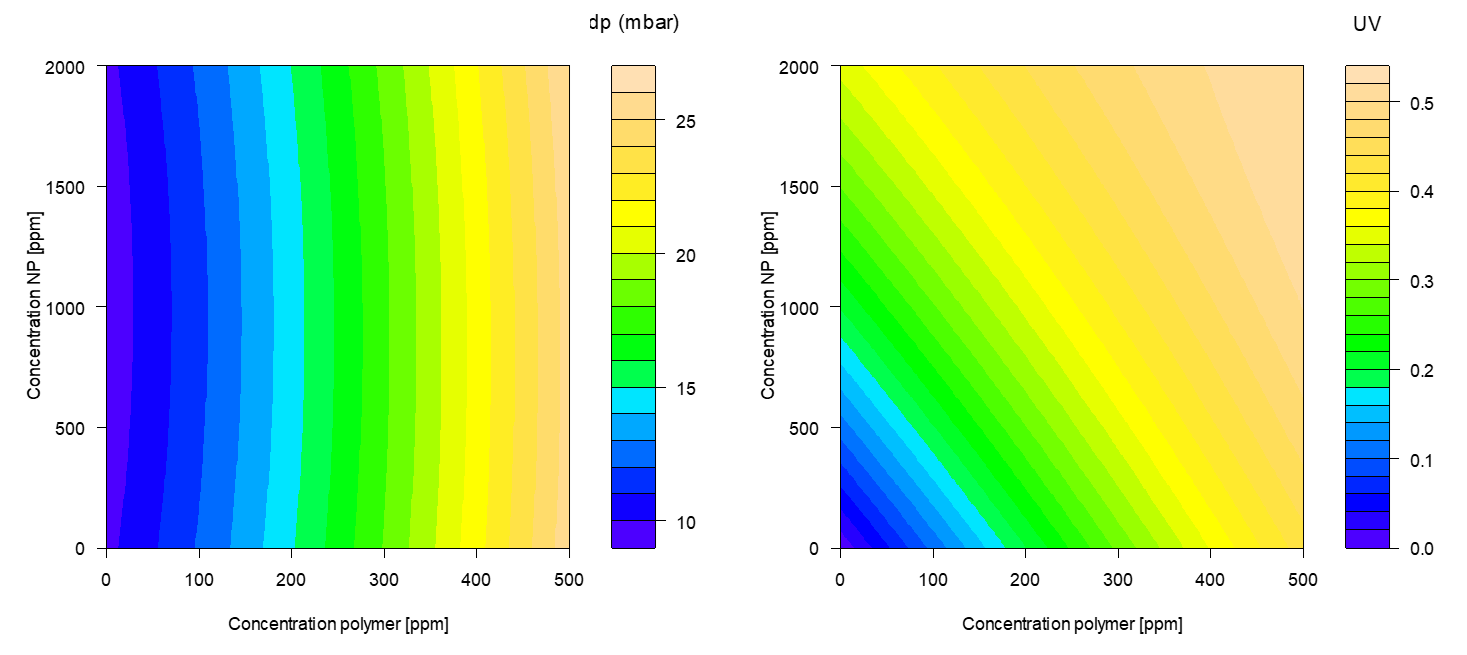
\includegraphics[width=\textwidth]{img/cht/uvDetector.png}
    \caption{Calibration models for pressure drop in viscometer (left) and UV absorption in UV detector (right). Polymer concentration varies along the horizontal axis and nanoparticle concentration varies along the vertical axis.}
    \label{cht:uv}
\end{figure}

Online measurements of polymer and nanoparticles using UV and refractive index measurements proved to be difficult. The reason for this is not revealed, but staining of the flow cells in the instruments is believed to be the most likely cause of these problems that also affected the accuracy in the results.

Nanoparticle and polymer solutions were prepared with \index{synthetic sea water} SSW as solvent (\textit{cf.} Table \ref{tab:sswComp}). Table \ref{tab:rockParams} summarizes the six different additive combinations used. Some of the experiments were repeated. In order to make a nanoparticle solution, Funzio-nano particles (FN-PEGMEA-100-141128) produced at SINTEF Materials and Chemistry were dissolved in SSW using a magnetic stirrer and then exposed to ultra-sonic bath a better dissolution. Finally, the solution was filtered through a 0.45 µm membrane filter. No significant increase in mass of the filters were detected. Partially hydrolyzed polyacrylamide (HPAM, FP 5115 VHM from SNF Floerger) was employed as the polymer. The molecular weight of the polymer is not exactly known but assumed in the order of 12 - 15 MDa. HPAM powder was dissolved in SSW with a propeller at 500 rpm followed by magnetic stirring. The polymer solutions, either at working concentrations or more concentrated solutions, were filtered through 5 cm long 500 mD Berea cores at rates up to 16 ml/min, but avoiding differential pressures over 20 bar. Two types of sandstone were used; Berea and Bentheimer. Basic core parameters are given in Table \ref{tab:rockParams}.

\begin{table} 
\small
\centering
\caption{Basic rock parameters and additives used in the experiments.}
\label{tab:rockParams}
\begin{tabular}{c c c c l } 
\toprule
\textbf{Exp. no.} & \textbf{Rock} & \textbf{Permeability} & \textbf{Porosity} & \textbf{Additive} \\ 
&& [Darcy] & [\%] & \\
\midrule 
1   & Bentheimer    & 2.74 & 23.1 & Nanoparticles\\
2   & Bentheimer    & 2.81 & 23.1 & Polymer \\ 
3   & Bentheimer    & 2.84 & 23.5 & Nanoparticles \& Polymer \\ 
4   & Berea      & 0.365 & 19.7 & NanoParticles\\
5   & Berea      & 0.288 & 18.6 & Polymer \\ 
5   & Berea      & 0.359 & 19.7 & Nanoparticles \& Polymer \\ 
\bottomrule
\end{tabular}
\end{table}




\section{Effect of in situ gelling on water flow} \label{sec:inSituGelling}
\subsection{Objective}
In this series of experiments, the effect of \textit{in situ} gel \index{\textit{in situ} gelling} formation on water flow was studied. The gel system used in the experiments was the system developed at SINTEF DMN. The chosen system was considered the most promising with regard to delayed gelation and formation of strong gels. The composition of the injected fluid is given in Table \ref{tab:injComp}. 
\begin{table} 
\centering
\caption{Composition of injected fluid}
\label{tab:injComp}
\begin{tabular}{c c c l } 
\toprule
\textbf{Constituent} & \textbf{Type} & \textbf{Mass} & \textbf{Comment}\\ 
&& [g] & \\
\midrule 
Polymer & Alcoflood 254S & 10.00 & MW $\thicksim$0.5 MDa, from BASF\\
Nanoparticles & FN-LA-65-170210 & 17.33 & 90.59 \% active matter \\ 
SSW & see Table \ref{tab:sswComp} & 490.0 &  \\ 
\bottomrule
\end{tabular}
\end{table}

\subsection{Experimental Setup}

The nanoparticles \index{experimental setup} were added to the polymer solution and stirred overnight with a magnetic stirring bar. The solution was then filtered through 8\micro m membrane filters using less than 2 bar overpressure. The loss of solids during filtration (measured for one solution) was 0.74 \% of active matter in the solution. This was obtained by weighing of the filters before and after (dried filters) filtration. The filters clogged during filtration and five filters were used during the filtration.

The experiments were carried out in the setup shown in Figure \ref{fig:experimentalSetup} but the various detecting systems except for the viscometer were bypassed. The experiments were done using 20 cm long Bentheimer sandstone cores at 80~\celsius~ and 4 - 5 bar back pressure.

The Bentheimer cores were initially characterized by measurement of porosity and permeability. Pore size distribution was not measured for the present cores. However, from previous measurements with Bentheimer sandstones with the same porosities, a pore size distribution curve was determined based on mercury intrusion measurements as shown in Figure \ref{cht:poreSizeDist}. The maximum of the curve was 33 \micro m, and only 11 \% of the pore throats were less than 10 \micro m (as seen from the raw data underlying the distribution curve).

\begin{figure}
    \centering
    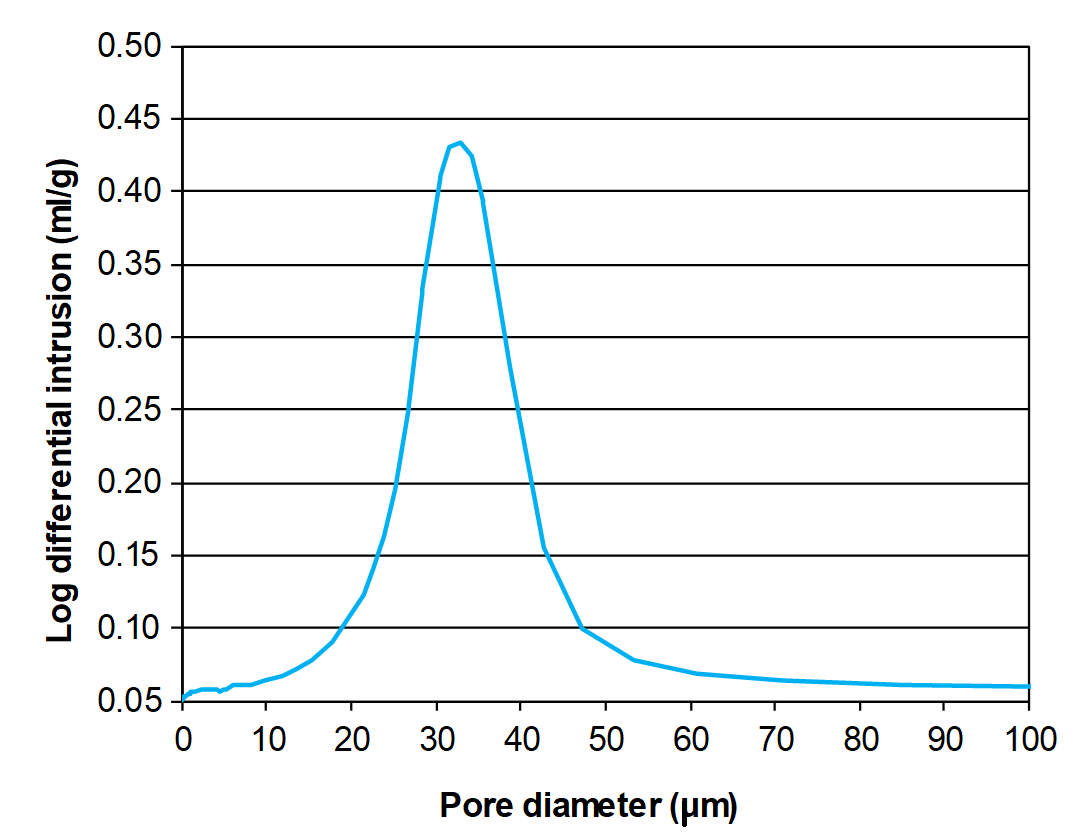
\includegraphics[width=.7\textwidth]{img/cht/poreSizeDist.png}
    \caption{Pore size distribution for Bentheimer sandstone}
    \label{cht:poreSizeDist}
\end{figure}

The first three experiments were conducted with increasing aging times for the chemical system
in the core. For each experiment, the pore volume and absolute permeability was first measured. Then, the chemical system was injected, followed by aging. After aging, SSW was injected at 30 ml/hr, and the experiments ended with a permeability measurement. During injection of the chemical system, samples of the produced fluid were taken early after breakthrough of the chemicals and at the end of the injection. The SSW injected prior to the polymer/nanoparticle solution was purged with argon and vacuum treated to remove oxygen from the solutions.

As differential pressures across the core increased significantly during injection of the identical nanoparticle/polymer solutions 2 more experiments were conducted. Experiment 4 was an injectivity test, pre-treating the injected solution by filtering it through a Berea sandstone. A last experiment was carried out by aging the solution with a more comprehensive pre-treatment, where the pH of the solution was reduced, and the solution was filtered through filters with smaller pore size.

\section{Effect of pH on in situ gelling}

When polymer and nanoparticles (lactamide POSS) solutions were mixed with synthetic sea water (SSW), the resulting solutions appeared somewhat turbid. The solutions used in the earlier injectivity experiments were therefore filtered before use. 

A more in-depth study of the formation of precipitates in mixtures of polymer and nanoparticles was required. To investigate the effect of pH on the properties of modified POSS and the resulting gels, a few tests were carried out at DMN. In addition to lactamide POSS (with 65 \% blocked amines), an imine POSS (100 \% blocked amines) was also included. The concentration of nanoparticles in the solutions were 3 wt. \% in SSW. The same polymer used was 2 wt. \% of Alcoflood 254, a 0.5 MDa HPAM from BASF.


\subsection{Effect of pH on modified POSS in SSW}
To investigate the influence of pH and ionic strength on the formation of precipitates, both POSS materials were dissolved in water and SSW. The initial pH of the solutions was over 9, indicating that all the solutions showed alkalinity, due to the primary/secondary amine in lactamide POSS and the secondary amine in imine POSS. The pH of the solution was adjusted to approximately 4 and 11 by HCl or NaOH, respectively.

Particle size and zeta potential of the solutions were measured under different pH.

\subsection{Effect of pH on mixtures of HPAM with POSS in SSW} \index{pH}
2 wt. \% HPAM solution was prepared in SSW. After the polymer was dissolved, approximately 3 wt. \% of imine POSS or lactamide POSS was added, respectively. The pH of the mixture was adjusted by adding HCl and NaOH. A similar behaviour as in the POSS solutions without HPAM was observed, where the precipitate dissolved when pH was adjusted to pH 4, indicating that acidic conditions are favourable to avoid precipitation.  

\section{Oil recovery with nanoparticles in injected water}
In measurements done at SINTEF outside the project it was found that addition of FN-nanoparticles could reduce the interfacial tension between brine and crude oil as well as changing the oil-water contact angle on several minerals. It was therefore a good idea to perform core flooding experiments in order to test a possible EOR effect. Two core flooding experiments were conducted where 1 wt.\% FN-PEGMEA-100 141128 was added tom SSW. 1.5 in. Berea sandstone cores were used in the experiments. The experiments were carried out in the setup shown in Figure \ref{fig:experimentalSetup} but the various detecting systems were bypassed. The produced fluids were collected in small samples using a fraction collector (Gilson Model 222) during the first part of the experiments, later larger collection vessels were used. The pump rate was 14 ml/hr. A back pressure of 6 bar was used.

Initial water saturation in the core was established by drop-wise adding 10 g of SSW on the core surface before the core was wrapped in Ni-foil and mounted in the core holder. The following day kerosene (IsoparL) was injected into the core until all air was removed. Oil permeability at initial water saturation was measured and the core holder was heated to process temperature. Basic core data and experimental conditions are summarized in Table \ref{tab:coreConditions5.13}.


\begin{table}
\small
\centering
\caption{Basic core data and some experimental conditions}
\label{tab:coreConditions5.13} % 5.13
\begin{tabular}{c l l l l l l } 
\toprule
\textbf{Experiment no.*} & \textbf{Length} & \textbf{PV} & \textbf{$\boldsymbol{K}_o(\boldsymbol{S}_{wi})$} & \textbf{$\boldsymbol{S}_{wi}$} & \textbf{Temp} & \textbf{Oil}\\ 
 & [cm] & [ml] & [Darcy] & [frac. PV] & \celsius & \\
\midrule 
2  & 0.221   &  7     & 2653     & 306      & 8.7  & IsoparL  \\
3  & 0.221   & 23     & 2580     & 5.2      & 493  & crude    \\ 
\bottomrule
\multicolumn{2}{l}{*\textit{Experiment 1 failed.}}\\
\end{tabular}
\end{table}